% This example An LaTeX document showing how to use the l3proj class to
% write your report. Use pdflatex and bibtex to process the file, creating 
% a PDF file as output (there is no need to use dvips when using pdflatex).

% Modified 

\documentclass{l3proj}
\usepackage{graphicx}
\usepackage{float}
\graphicspath{ {./images/} }


\begin{document}

\title{Thales Sensor Mapping Demonstration Software}

    \author{Krasimir Ivanov\\
        Mohammad Atbaan Akhtar \\
        Shahzeb Zafar \\
        Shayam Nitin Bhudia \\
        Vrinda Sharma\\ 
        Krishang Patney\\}

\date{April 9, 2021}

\maketitle

\begin{abstract}

This paper presents a case study of the development of a sensor mapping software.   
<Add more here.>

\end{abstract}

%% Comment out this line if you do not wish to give consent for your
%% work to be distributed in electronic format.
\educationalconsent

\newpage

%==============================================================================
\section{Introduction}

This paper presents a case study of the development of a sensor mapping software. The application takes data from a sensor system like the SOPHIE LITE Electrical External ICD device. The application takes in the scan data and maps it onto a 3D or a 2D map to visualize the scanned data. Furthermore, the mapping function can simulate the sensor system.

The paper begins with some background information about our customer and their proposal (section 2 \& 3). It then delves into details about our main application followed by a thorough recount of the software development process (sections 4 \& 5). 

This is followed by our reflection about the project and key insights gained throughout the six to seven months of development (section 6). We finally conclude it with a brief look at the various software development practices we adopted and how closely our project’s progress was tied to the Professional Software Development course (section 7).

%==============================================================================
\section{Our Customer}

Thales Group is a French multinational company, founded in December 2000, that designs and builds electrical systems and provides services for the aerospace, defense, transportation, and security markets.\cite{wikipedia-Thales} The proposal that was given to our team, CS01, by the company’s UK branch. Thales UK approached the University of Glasgow Computer Science department to task a student development team to build a proof of concept of sensor data visualization and simulation application.

Our customers consisted of Ian James, Iain Carrie, Matt Tucknott, and Christopher Dickson. Ian acted as our main point of contact and sponsor on behalf of Thales. Iain is the Project Technical Lead for Urban Canyon, one of Thales’ many ongoing projects, and was the main beneficiary of our application. Matt is a Thales Technical Expert on Geographic Information Systems (GIS)  and has had over 20 years of experience in the field as well as 29 years of Java and C++. Christopher is a Thales Algorithms Engineer with over 19 years of software experience and has 10 years of experience with image processing.

The way our customer’s team was structured was that Ian would be our main liaison. Most of our conversations were with him and he was the first to be informed of any issues or scheduling details for meetings from our end. Iain was the one who approved of or suggested many of our application’s features earlier on during development while Christopher and Matt provided development support. Matt in particular was integral for fixing one of the major roadblocks we faced over halfway through development (more on this later). 

%==============================================================================
\section{The Project Proposal}

Thales UK was looking for software to support a LIDAR sensor system with mapping information in 2D and 3D with potential real-time information update capability. Their long-term aim was to bring autonomous and manned platforms closer together with the integrated sensor and mapping software they proposed. The proposed project specification first aimed to develop a simple overlay of a target locator sensor on a map and then aimed to extend the integration to be 3D. The client stated that they were not constraining the development team on what technologies to use, however they would prefer that the mapping tool and the sensor suite be integrated to better aid their aim for the software to cope with a wide variety of situations.

The produced software solution is an open-source MIT licensed prototype, therefore a patent will not be sought. The main purpose and use of the software product are to provide proof of concept. The product will not be deployed into production, only used for demonstration purposes. The goal of the project proposal was to explore the technologies needed to develop such an application, what resources it needs, and to implement a prototype solution.

They stated that their goal for the first couple of iterations was to research available technologies for the framework of the application and what modules to use for the map and the mapping of the sensor information. This was aided by their recommendations on technologies as well as the availability of their software professionals, mapping, and sensing experts. After careful consideration and ranking of frameworks, the team initially settled on using the framework ElectronJS with Cesium, a 3D geospatial modeling tool, to start with.

%==============================================================================
\section{The Application}

Before we can discuss the application, we need to know the minimum viable product our customers expected. At the start of the first sprint, after our first meeting with the customer, we gathered the three major tasks, which would result in being the minimum viable product, with each of being split couple of sub-tasks. They were:

Task 1 - Establish a relationship between video and 2d (ground plane) map:
\begin{itemize}
	\item Task 1a: Populate a 2d radar plot (azimuth vs range) with detections obtained from a video. Assume 2d bounding box in the image, known calibration/pose of the camera, and known distance to object.  
	\item Task 1b: Annotate a 2d ground plane map with detections obtained from a video. As above, but plot on an open-source map based on known vehicle position/orientation. 
\end{itemize}

Task 2 - Establish a relationship between video and 3d map:
\begin{itemize}
	\item Task 2a: As Task 1b but remove the assumption of known distance to target and plot result on 3d map (or 2d ground projection of 3d map). Distance to target should be automatically determined by intersecting bearing from known bounding box with a ground plane as defined by the 3d map. Report the range to target.
	\item Task 2b: Project all visible rays from a camera onto 3d map and display total visibility from the current position. Assume knowledge of camera calibration, camera field of view, and camera/vehicle pose. 
\end{itemize}

Task 3 - Plot features from 3d map onto a video feed:
\begin{itemize}
	\item Task 3a: For an object positioned on the 3d map, determine and display its location in the video feed. Assume known calibration/pose of camera + known vehicle position. 
	\item Task 3b: Combining Tasks 2b and 3a determine whether the object identified in 3d map is visible to the camera and if not highlight that it is a hidden target.   
\end{itemize}

Along with this, we had also been asked to provide additional functionalities if time permits, they also requested to make the application open-source. To fulfill our tasks and carry out the request, we were recommended several APIs and software by our customers. Initially, we settled on CesiumJS and ElectronJS but over halfway through the project’s development lifecycle, we switched to our ArcGIS + JavaFX based application due to the limitations of our earlier approach, now called ThalesArc.

\subsection{ElectronJSApp}
This application had been made by combining a couple of technologies. The most notable being CesiumJS, which is an open-source JavaScript library for creating static or dynamic 2D and 3D maps,\cite{cesiumJS} it supports for creating multiple maps which we deemed ideal for the intended use. Secondly, the front-end framework we used was Bootstrap, which allows for creating responsive websites, with a grid system, extensive prebuilt components, and powerful JavaScript plugins\cite{Bootstrap}. 

Both these technologies are combined and packaged under ElectronJS an open-source software framework based on Chromium, which runs under the open-source JavaScript server runtime environment called Node.js\cite{Node.js}. 

This application is versatile, as Cesium can provide most of the data sets for 2D and 3D map features, we'd require. On top of this, the people at Cesium regularly update the extensive documentation with a sandbox feature to showcase their predominant features and how they can be integrated into a web-based application. A python script was first used to simulate sensor data and plot points on the map, but this was later scrapped in favour of an Android application we developed which could send actual geographical data gathered from a phone’s GPS to the application by utilising Web Sockets, this makes it possible to communicate between the application and user.

Cesium is a great API for displaying geospatial information within a web browser, making it lightweight, and easy to distribute on a massive scale, meaning it'd be great for displaying static data which does not change a lot, however, one of its major drawbacks is not being able to utilize the GPU on a computer, which would be the main platform for our application to be run on, this meant that having a constantly updating data stream would bog down the performance of the application, hence not being satisfactory enough for our vision of the product.

On top of the above-mentioned issues, we were also unable to project visibility rays within the 3D world hence not knowing where our targets would be located as they would be rendered in without having geospatial information attached to it. One of the solutions that'd allow us to overcome this roadblock would be to purchase the Cesium ion SDK licence, therefore making it proprietary software and being over-budget.

These issues, combined with the application not deploying on anything but Windows, meant that we had reached the end of the road with Cesium and had to find a new approach to our project.

\subsection{ThalesArc}

ArcGIS Pro was our answer to Cesium’s shortcomings. This is a geographic information system software developed by the Environmental Systems Research Institute (Esri) which supports an API based on a 64-bit architecture and combines support for 2D and 3D applications, used for geospatial processing programs. Making it a great contender to the previously maintained ElectronJSApp application. ArcGIS Pro was integrated onto the JavaFX client application platform supporting cross-platform development and releases.

The new application was everything we had hoped to achieve but failed to with the ElectronJSApp. This new API allowed us to project the field-of-view rays from the camera, whilst utilising the GPUs capabilities, hence allowing us to move the field-of-view cone around on the map just like a senor would be based on the geographic coordinate system.

Like before, a python script had now been modified to allow for sending JSON packets to the application which then converted them to Sensor objects, allowing us to have simulated data streams for plotting new user coordinates and target coordinates if given. However, due to time constraints, we were unable to further develop the Android simulator application to support the new ThalesArc app.

Whilst also completing the minimum viable product we were able to implement a few extra features which the customer had mentioned within their product requirements draft. This included adding a detailed log of all the targets being shown to the user, functionality of loading, creating, and saving these logs within the user's directory, and also additional features which can be further developed if wished by the customer, such as having target paths, which can be abstracted to also display the users routing.

\subsection{Application Comparisons}

Whilst writing down a few key features of the applications mentioned above would be a good enough explanation to a GIS expert, it can also easily confuse someone new to mapping technologies. Hence providing a more detailed explanation and comparison between the applications.

To realize our vision for the application it's beneficial to take a look at the wireframes developed within the first sprint of the software development lifecycle, which set out a concrete foundation for what the app would look like. As we can see in Figure 1, the wireframe is split into a few components, the left side is split off to log all the targets on the map, and a few more options for the user to choose between features and also displaying the current user location. The right side hosts the map which displays the field of view cone with the dead of ground information and users position.

\begin{figure}[!h]
    \caption{Sample wireframe}
    \centering
    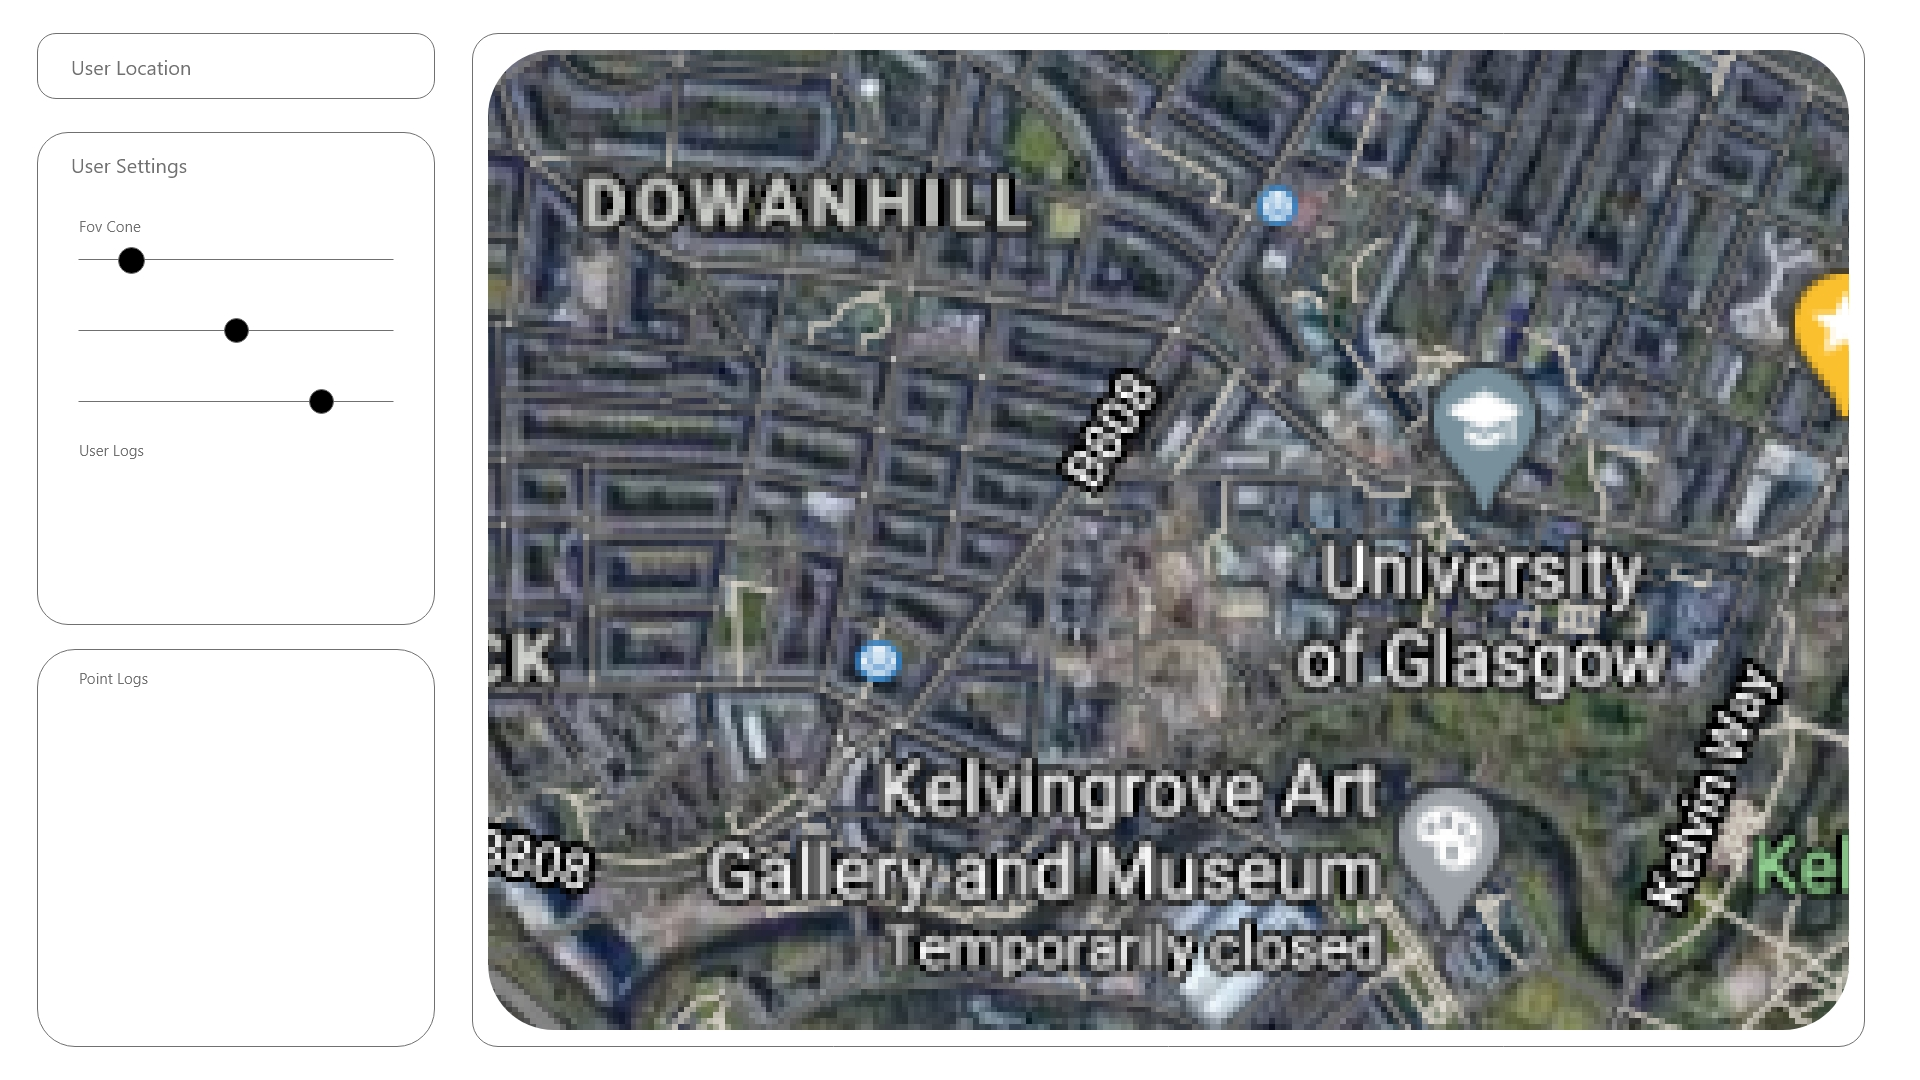
\includegraphics[width=\textwidth]{wireframe.jpg}
\end{figure}

With the development of the product being split into two applications, starting with the first, ElectronJSApp. We've provided a 2D map starting in Glasgow. This application fulfils the customer's Task 1, which establishes a relationship between what a sensor can see which then gets plotted onto the 2D map, for example, we could spawn randomly generated points on to the map and a fixed user location. However, a big issue we faced is the points get generated onto a single graphic layer, combined with the map, resulting in computationally expensive graphic processing, which a web browser is not capable of. Especially if we wanted to have the constant stream of data coming in and updating the user's current location graphically while doing other processes. 

This segways into the second application we've developed as mentioned before which uses the ArcGIS Pro API. Which works in a more industry-standard fashion for mapping applications, where it uses data layers as a mechanism to display geographical datasets. The sample dataset we've used is located in Brest, France as it's provided by ArcGIS Pro out of the box.

\begin{figure}[!h]
    \caption{Example of layers in ArcGIS}
    \centering
    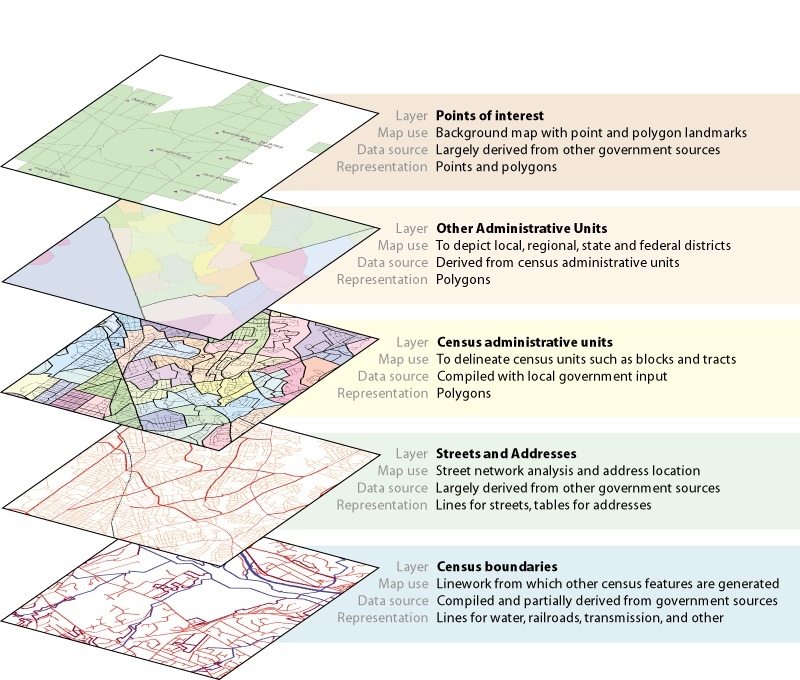
\includegraphics[width=\textwidth]{GISLayers.jpg}
\end{figure}

In figure 2 we can see different layers being are used in the image to display a few map features. Taking a note from this example we've personally used 3 main layers, one for each, the user, the targets and the field of view, with other additional layers for extra features. This allows us to dynamically or statically update each layer on its own hence reducing lag, and allowing us to use GPU resources to render the graphic layers in dynamically in real-time. 

\begin{figure}[H]
    \caption{ThalesArc line of sight visibility feature}
    \centering
    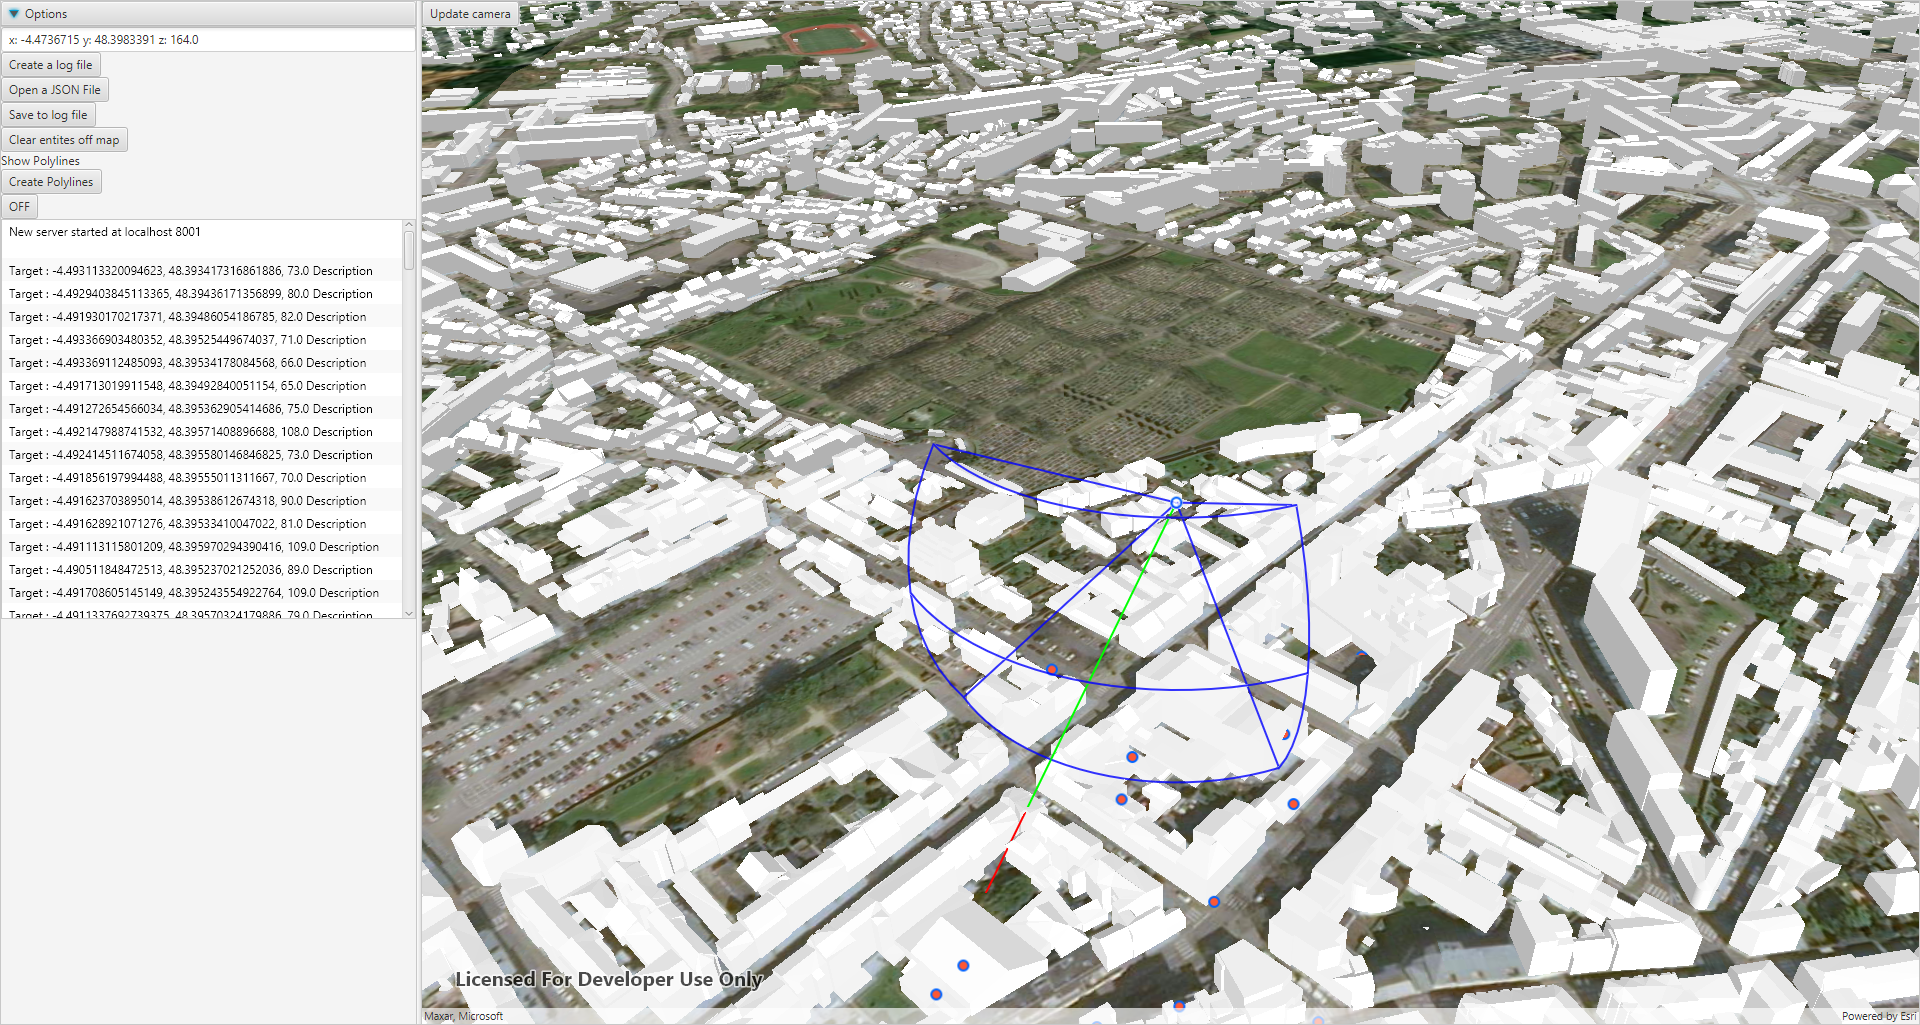
\includegraphics[width=\textwidth]{ArcGISLOS.jpg}
\end{figure}

Figure 3 showcases the feature, where we try and process the line of sight from a user to a target, which works by highlighting the line green if the point can be seen from the user and red if not.

\begin{figure}[H]
    \caption{ElectronJSApp line of sight visibility feature}
    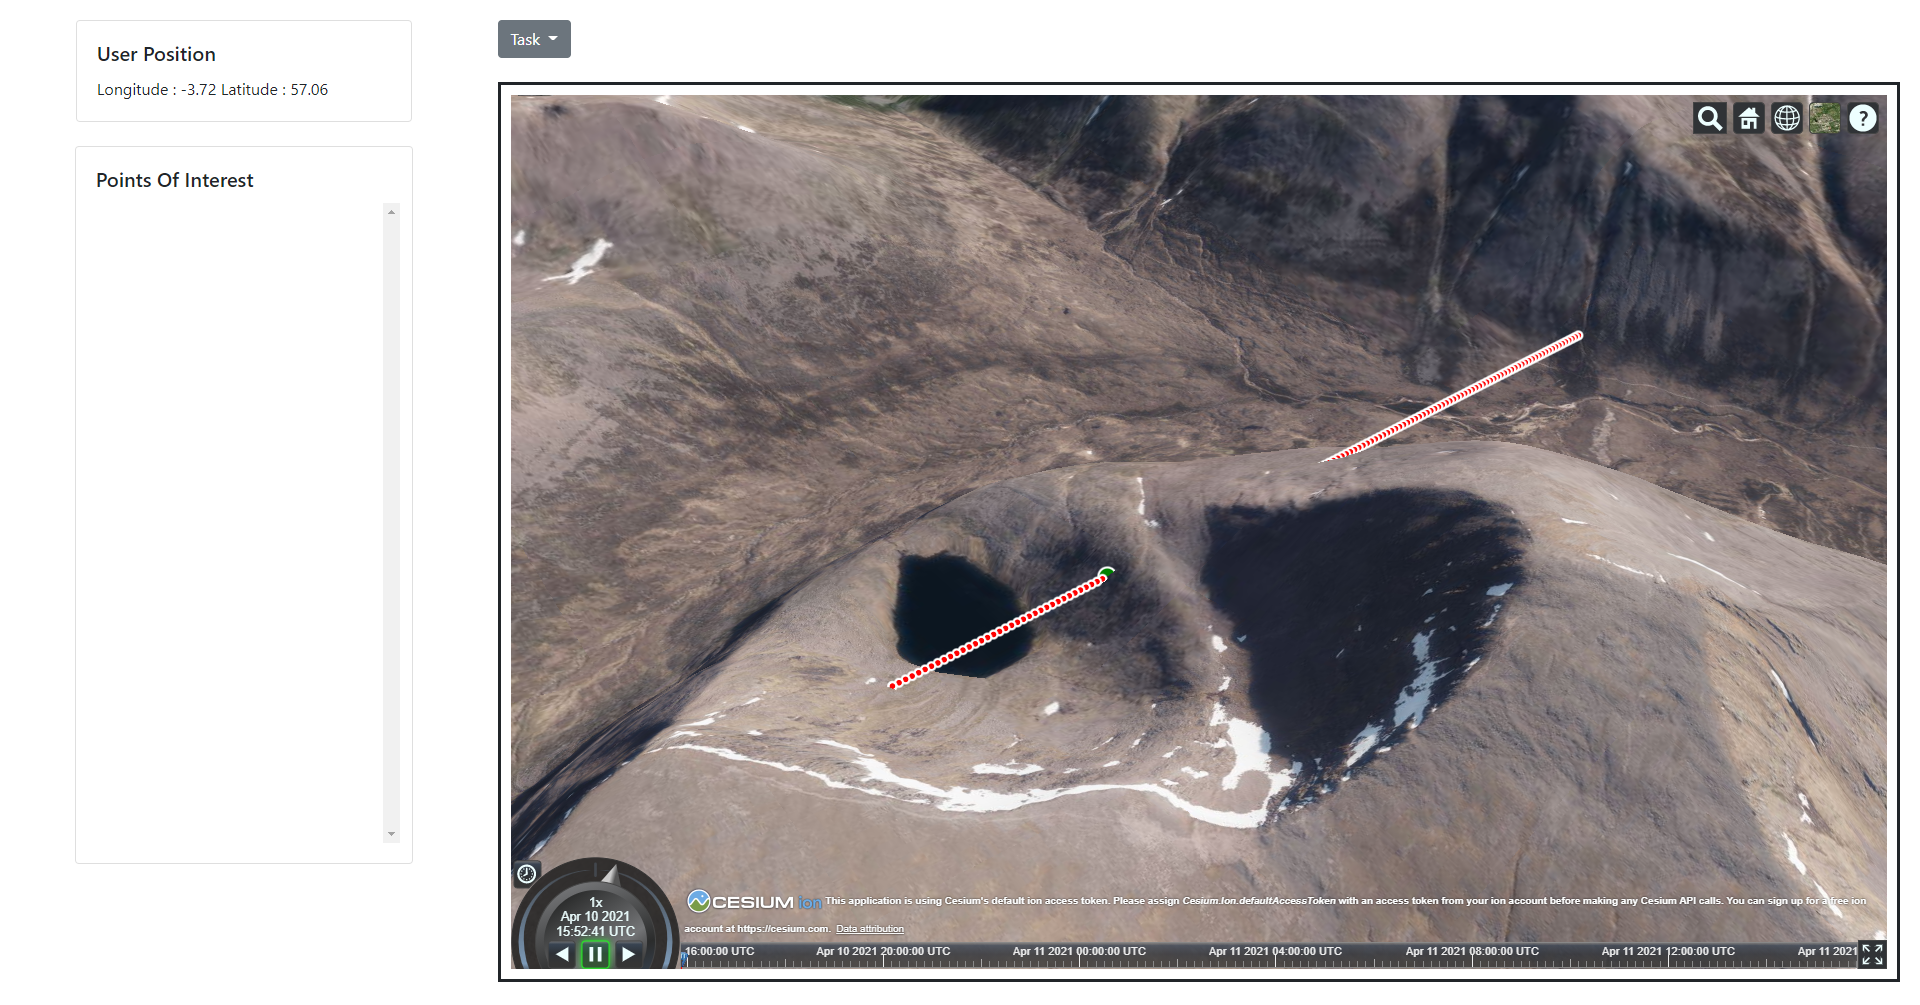
\includegraphics[width=\textwidth]{ElectronJSLOS.jpg}
\end{figure}

Trying to achieve this functionality in the ElectronJSApp required us to create many points in between the user and map to see whether or not it'd intersect with its surrounding terrain as seen in Figure 4. Whilst doing this process, the application gets resource hungry and start to bog down its overall performance. 

Other miscellaneous features that have been included are vector representation for targets, this can be abstracted to be used for the user's route or be disabled upon the users wish. Users can go back to the original user location by clicking the "Update Camera" button, they also have the freedom to create, save and update the log files which are stored in the "LogFiles" directory, for which a sample file has also been provided for demonstration.

%==============================================================================
\section{Software Development Process}

As detailed in the Project Proposal section of the report, a requirement was given to the development team by Thales UK outlining a support software for a sensor system. The requirement stated that the purpose of the application was to be a demo, that it would never be used as a live product. The development team kept this in focus throughout the planning and execution of the project. Furthermore, it is worth noting that the development team and the customer agreed that the produced software repository will be under an open source licence also called the MIT licence, it grants any person who obtains a copy of the software and associated files the right to use, copy, modify, merge, distribute, publish, sublicense, and sell copies of the software. \cite{MIT_License}

The development process the team used can be broken down into 4 sections. First, understanding the requirements given and formulating an action plan. Second, implementing the action plan, which was the development phase, that continued in parallel with the third phase. Third, testing the developed product. The fourth and last phase was the delivery of the produced software to the client. 

The implementation of the software product started with choosing a technology to work with, that was capable of supporting the proposed requirements and functionalities. Once the technology and the framework were chosen the development team proceeded to implement the requirement in a procedural order. The development was broken into cycles or sprints. Throughout the whole duration of the project, there were 5 sprints, each sprint lasting 4 weeks. During the sprints, goals were set to be achieved by the team and to facilitate achieving the overarching sprint goal, stories or tasks were set up and were assigned to the members of the development team. 

At the end of a sprint, there was an evaluation of the work that had been done, a code review, and a retrospective was held to reflect on the sprint and the performance of the team members as well as determining if the goals of the sprint had been met. During the retrospective, the team listed the good, the bad and the ok elements of the sprint. The retrospectives were a crucial part of the team dynamic and keeping the team on track to achieve the main goal of the project, the delivery of the software product while assuring quality. 

The other method that was used to ensure the consistent quality of the software and to root out bugs was testing. The two methods that were used for testing was the traditional manual way, user testing; the other was an automated, robust method, Unit testing. The implemented tests had decent software coverage, however, Unit testing was not used for UI testing, therefore that was done manually by the team's testers. Gitlab runners were used to implementing Unit testing for both the core applications and the CI/CD pipelines. The tests were run as jobs on a UNIX machine. The development team planned on having Unit test jobs running across the entire application, however, due to unforeseen hurdles during the development test runners could not be set up for the display drivers. This meant the development team could not set up pipelines successfully for the ElectronJSApp, however, they were successful in creating the ThalesArc application pipeline. 

Once the project deadline had been passed, the delivery of the completed application had begun, where we set up a release branch, accessible by the customers as they had previously been added onto the repository. From here both our applications have installation instructions provided for the customer to install the demonstration applications onto their servers, hence being fully handed over. Additionally the team has taken no further responsibility to maintain or develop the application. 
%==============================================================================
\section{Reflection and Insights}

Although there were many ups and downs throughout this project and many days of frustration, it was very insightful and a great learning experience. Here are some of the things the members of our team have to say regarding everything:

Krasimir: The project showed me the value of working in a team for a longer period of time. Furthermore, I learned how to go from a general project description to a complete application. I also improved my ability to gather requirements from customers which is vital in the industry.

Atbaan: This project has helped me understand how there is so much more to being a software developer than just programming. It taught me how to interact with customers and my teammates over a long time period and it gave me "real-world experience" while still studying at the university.

Shahzeb: My experience with the team project has been quite good. I met and got along with new people who I very much enjoyed working with. I got to experience some of the hardships that take place during the development of any software and gained a new appreciation for software developers. Most importantly, I learned a new set of skills that will come in handy should I ever take up software development in the future.

Shayam:

Vrinda: This project really helped me understand the intricacies of the software development process which is crucial for working in the industry. Working with a team for over 6 months helped me understand the importance of teamwork and dividing the work efficiently to achieve more in less amount of time.

Krishang: The project helped me take a look into what software engineering practices could look like for a product that aims to be served as a demonstration tool, whilst also giving an insight into what it takes to create a product from the ground up while only being given a description of its potential features.



%------------------------------------------------------------------------------
\section{Conclusions}



%==============================================================================
\bibliographystyle{plain}
\bibliography{dissertation}
\end{document}
